
% ----- ASY SETUP ----------------------------
\begin{asydef} 
defaultpen(fontsize(10));
settings.outformat="pdf";
usepackage("amsmath");
usepackage("amssymb"); 
usepackage("mathpazo_modified");
texpreamble("\renewcommand{\vec}[1]{\mathbf{#1}}");
texpreamble("\let\e\relax");
texpreamble("\DeclareMathOperator{\e}{e}"); 
import x11colors;
pen softblue = rgb(0.92,0.95,0.99);
pen softred = rgb(0.99, 0.92, 0.91);
pen softyellow = rgb(0.98, 0.98, 0.9);
pen softgreen = rgb(0.96, 0.995, 0.98);
settings.render = 8;
\end{asydef}

\newsavebox{\asybox}
\def\asydir{asy}

%---- PRINT AUTHOR INFO ------------------
\makeatletter                       
\def\printauthor{%                  
  {\large \@author}}              
\makeatother
\author{%
  {\Large \textit{Samuel S.\ Watson}} \\ \vspace{2mm} {sswatson@brown.edu}
}

%----- SIDE ICONS ------------------------
\newcommand{\milink}[3][-7.5mm]{\sidenote{\href{http://mathinsight.org/#2}{\mi} on #3}[#1]}
\newcommand\cocalc[1][-2pt]{\raisebox{#1}{
\includegraphics[width=12pt]{figures/cocalc_new}}}
\newcommand\tbob[1][-2pt]{\raisebox{#1}{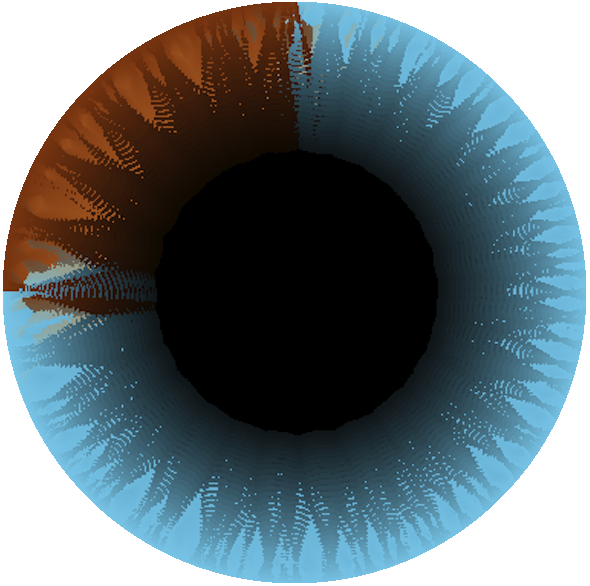
\includegraphics[width=12pt]{figures/3b1b_new}}}
\newcommand\mi[1][-2pt]{\raisebox{#1}{
\includegraphics[width=12pt]{figures/mathinsight}}}

%This cover art is taken from 
%http://tex.stackexchange.com/questions/85904/showcase-of-beautiful-title-page-done-in-tex

\definecolor{titlepagecolor}{cmyk}{1,.60,0,.40}

\newcommand\titlepagedecoration{%
\begin{tikzpicture}[remember picture,overlay,shorten >= -10pt]

\coordinate (aux1) at ([yshift=-15pt]current page.north east);
\coordinate (aux2) at ([yshift=-410pt]current page.north east);
\coordinate (aux3) at ([xshift=-4.5cm]current page.north east);
\coordinate (aux4) at ([yshift=-150pt]current page.north east);

\begin{scope}[titlepagecolor!40,line width=12pt,rounded corners=12pt]
\draw
  (aux1) -- coordinate (a)
  ++(225:5) --
  ++(-45:5.1) coordinate (b);
\draw[shorten <= -10pt]
  (aux3) --
  (a) --
  (aux1);
\draw[opacity=0.6,titlepagecolor,shorten <= -10pt]
  (b) --
  ++(225:2.2) --
  ++(-45:2.2);
\end{scope}
\draw[titlepagecolor,line width=8pt,rounded corners=8pt,shorten <= -10pt]
  (aux4) --
  ++(225:0.8) --
  ++(-45:0.8);
\begin{scope}[titlepagecolor!70,line width=6pt,rounded corners=8pt]
\draw[shorten <= -10pt]
  (aux2) --
  ++(225:3) coordinate[pos=0.45] (c) --
  ++(-45:3.1);
\draw
  (aux2) --
  (c) --
  ++(135:2.5) --
  ++(45:2.5) --
  ++(-45:2.5) coordinate[pos=0.3] (d);   
\draw 
  (d) -- +(45:1);
\end{scope}
\end{tikzpicture}%
}
